\section*{Cíle laboratorního cvičení}
\begin{itemize}
  \item Seznámení se se signalizačním protokolem SIP.
  \item Navázání komunikace VoIP typu Peer-to-peer pomocí signalizace SIP.
  \item Komunikace VoIP pomocí signalizace SIP přes ústřednu.
\end{itemize}

\section*{Základní instrukce}
\begin{itemize}
  \item Zkontrolujte připojení sluchátek s mikrofonem k počítači. 
  \item Přihlašte se do CentOS (F3) jako uživatel {\tt user} s heslem {\tt user4lab}.
  \item V pravé horní části obrazovky {\bf zkontrolujte nastavení zvuku}. Ověřte funkčnost sluchátek a mikrofonu, nastavte optimální hlasitost. 
  \item Otevřete si příkazovou řádku pro uživatele {\tt user}.
  \item Otevřete si příkazovou řádku pro uživatele {\tt root} (příkazem {\tt su}).
  \item V případě potřeby si otevřete další terminál v novém okně.
  \item Vyčistěte si pravidla ve firewall pomocí příkazu {\tt iptables --flush}.
\end{itemize}

\section{Komunikace VoIP typu peer-to-peer: práce ve dvojicích}
V této části laboratoře nastavíte a analyzujete VoIP komunikaci se svým sousedem bez použití ústředny (spojení typu peer-to-peer).

\begin{enumerate}
    \item V terminálu uživatele {\bf user} zapněte klienta VoIP se jménem Jitsi (příkaz {\tt jitsi \&}).
    \item V menu {\bf Tools} $\rightarrow$ {\bf Options} $\rightarrow$ {\bf Accounts} přidejte nový účet. V poli {\bf Network} zvolte možnost {\tt SIP}. Jako {\bf SIP id} použijte Váš {\tt xlogin}, heslo nezadávejte.
    Vytvoření účtu potvrďte tlačítkem {\bf Add}. Zkontrolujte, že se vytvořil {\it RegistrarLess SIP} účet.
    \begin{figure}[h!]
    	\centering
    	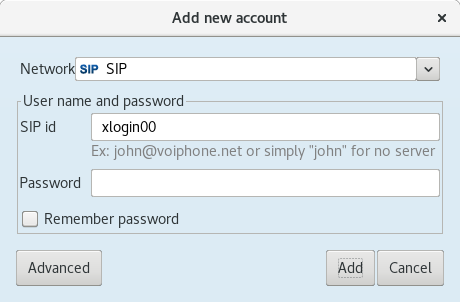
\includegraphics[scale=0.5]{img/account_p2p.png}
    	\caption{Nastavení účtu SIP.}
    	\label{fig:sip_account}
    \end{figure}
    \item V terminálu uživatele {\tt root} spusťte síťový analyzátor Wireshark (příkaz {\tt wireshark \&}). Začněte zachytávat pakety na rozhraní {\tt enp2s0}.
    \item Nastavte display filtr tak, aby zobrazoval pouze protokol SIP.
    \item V hlavním okně programu Jitsi zadejte do pole {\it Enter name or number} IP adresu Vašeho souseda: {\bf 10.10.10.xxx}.
    \item Zavolejte sousedovi stisknutím zeleného telefonu. Vyzkoušejte, zda se navzájem slyšíte, po chvíli hovor ukončete.
      (V případě problémů se zvukem zkontrolujte, zda není v operačním systému ztlumen mikrofon či audio výstup, případně zkontrolujte nastavení zvukových zařízení v aplikaci Jitsi, menu Tools $\rightarrow$ Options $\rightarrow$ Audio.) 
    \item Proveďte analýzu navázaného spojení v analyzátoru Wiresharku. Využijte menu {\bf Telephony $\rightarrow$ VoIP Calls}, kde uvidíte jednotlivé zaznamenané hovory. Vyberte příslušný hovor a zobrazte jeho průběh volbou {\bf Flow}.
    \item Zakreslete spojení do protokolu. Uveďte použité přenosové protokoly, IP adresy, porty a kodeky.
\end{enumerate}
Názvy a čísla podporovaných kodeků si strany vymění protokolem SDP, který je zapouzdřen v těle příkazů {\bf INVITE} a {\bf OK}:
\begin{figure}[h!]
  \centering
  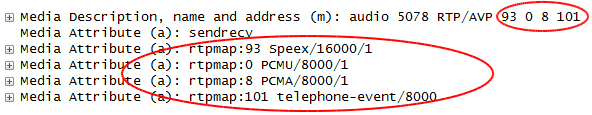
\includegraphics[scale=0.65]{img/3a.png}
\end{figure}

\noindent Informace o vybraném kodeku získáte z hlavičky paketu RTP {\bf Payload type}.
\begin{figure}[h!]
  \centering
  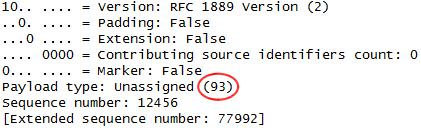
\includegraphics[scale=0.65]{img/3b.png}
\end{figure}


\section{Komunikace VoIP přes ústřednu SIP: práce ve dvojicích}
Nakonfigurujte si nový účet v aplikaci Jitsi, který bude komunikovat přes ústřednu SIP s VoIP doménou {\tt isa-lab.cz}. Jméno účtu bude {\tt userXX@isa-lab.cz}, heslo {\tt hesloXX} a vaše telefonní číslo {\tt 10XX}, kde {\it XX} je číslo Vašeho počítače. 

\subsection{Registrace VoIP klienta na ústředně}
\begin{enumerate}
    \item Spusťte znovu zachytávání paketů v aplikaci Wireshark.
    \item Vraťte se do hlavního okna aplikace Jitsi a otevřete menu {\bf Tools} $\rightarrow$ {\bf Options} $\rightarrow$ {\bf Accounts}.
    \item Vytvořte nový účet. V poli {\bf Network} vyberte opět možnost {\tt SIP}. Tlačítkem {\bf Advanced} zvolte pokročilou konfiguraci.
    \item V poli {\bf SIP id} nastavte hodnotu {\tt user{\bf XX}@isa-lab.cz}, heslo {\tt heslo{\bf XX}}, kde {\tt\bf XX} je číslo Vašeho počítače. Do pole {\tt Display Name} zadejte své jméno a příjmení (bez diakritiky), viz obrázek \ref{fig:registration1}.
      \begin{figure}[h!]
        \centering
        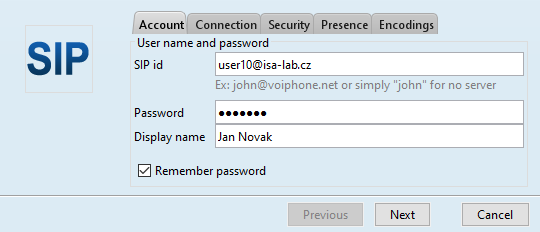
\includegraphics[scale=0.7]{img/jitsi-registration1c.png}
        \caption{Vytvoření účtu.}
        \label{fig:registration1}
      \end{figure}
    \item V záložce {\bf Connection} nastavte v poli {\bf Proxy} IP adresu SIP serveru na hodnotu {\tt 10.10.10.222}. Číslo portu zadejte {\tt 5060}, viz obrázek č. \ref{fig:registration2}. 
      \begin{figure}[h!]
        \centering
        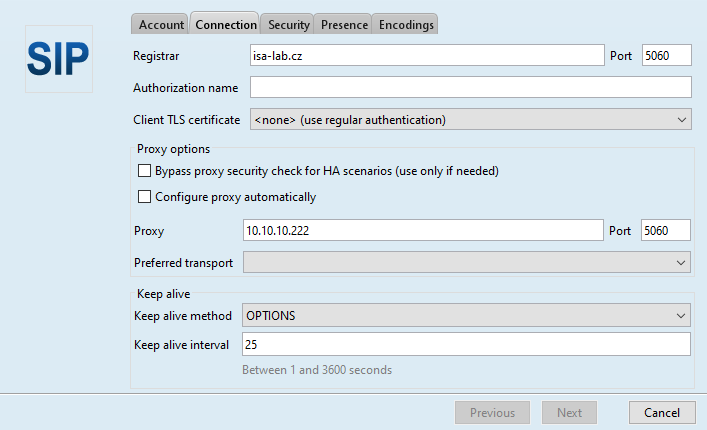
\includegraphics[scale=0.7]{img/jitsi-registration2b.png}
        \caption{Konfigurace adresy ústředny.}
        \label{fig:registration2}
      \end{figure}
    \item Tlačítkem {\bf Next} a {\bf Sign in} provedete registraci na ústředně.
    \item  Pokud jste vše nastavili správně, v seznamu účtů v menu {\bf Tools} $\rightarrow$ {\bf Options} uvidíte účet ve stavu {\bf SIP Online}. {\it V případě neúspěchu účet odeberte a znovu přidejte. Pokud ani toto nepomohlo, ukončete Jitsi a postupujte znovu od kroku 1, případně konzultujte problém se cvičícím.}
    \item Odhlašte se od ústředny v okně pro správu účtů pomocí kliknutí na
      zaškrtávací tlačítko účtu.
    \item V programu Wiresharku analyzujte průběh přihlášení k ústředně a
      odhlášení od ústředny. Zaměřte se na příkazy {\bf REGISTER} a jejich
      odpovědi. Jiné zprávy, jako je PUBLISH, SUBSCRIBE, OPTIONS neslouží k
      přihlášení klienta k ústředně. Do protokolu zakreslete průběh registrace. Z hlavičky SIP (položky From, To, Contact, User-Agent, Server, Expires) určete logickou adresu uživatele (User URI), adresu připojení (Device URI), jméno a verzi VoIP klienta, jméno a verzi SIP serveru, maximální dobu přihlášení. Čím se liší obsah paketu {\bf REGISTER} při přihlášení a odhlášení uživatele?
\end{enumerate}

\subsection{Analýza hovoru přes ústřednu}
\begin{enumerate}
  \item Znovu se zaregistrujte k ústředně, viz předchozí část 2.1.
  \item Otestujte spojení voláním na linku {\tt 123}. V případě správného nastavení vám systém přehraje automatickou kontrolní hlášku. 
    \item Obnovte zachytávání paketů v aplikaci Wireshark.
    \item Zavolejte svému sousedovi. V hlavním okně Jitsi zadejte telefonní číslo Vašeho souseda ve formátu {\tt 10xx}, kde {\it xx} je číslo počítače.
    \item Proveďte analýzu odchycených paketů v programu Wireshark. Zaměřte se na příkazy {\bf INVITE}, {\bf OK} a {\bf ACK}. Z hlaviček {\it From} a {\it Contact} určete User URI a Device URI volající i volaného.
    \item Z protokolu SDP určete IP adresu a port pro přenos hlasových dat na straně volajícího i volaného. Určete použitý kodek. 
    \item Průběh spojení zakreslete do protokolu a zapište požadované hodnoty. {\it Poznámka: každý student zakreslí svou část hovoru, kdy volal sousedovi.}
\end{enumerate}

\subsection{Telefonování přes ústřednu do jiné VoIP domény}
\begin{enumerate}
    \item Na telefonu zvolte telefonní číslo na linku VUT s číslem 54114 1046.
    \item Oznamte vyučujícímu, že jste skončili s prací a odevzdejte mu ke kontrole vypracovaný protokol. 
    \item Podle pokynů vyučujícího zkontrolujte a opravte případné nepřesnosti v protokolu. 
\end{enumerate}

\section{Ukončení práce v laboratoři}
\begin{itemize}
  \item Počítač vypněte spuštěním skriptu {\tt /root/isa4/clean} (jako uživatel {\bf root}).
\end{itemize}
